\chapter{Internet Protocol}
\label{chap:ip}

\section{\acs{IP} addresses}
\label{sec:ip-addresses}
   
\paragraph{32 bits}
An \acs{IP} version~4 address is a 32-bit number meaning the computer uses 32~bits or four octets to store the \acs{IP} version~4 address in memory.
What these four octets mean, depends on how we want to interpret them.
For example, the following 32~bits can be interpreted as the number \numprint{1113945185}.%
   \footnote{You can also interpret these four octets as the string `Beta' when using the \acs{ASCII} character table for the conversion.}
\begin{center}
\lstinline{0100 0010}\quad\lstinline{0110 0101}\quad\lstinline{0111 0100}\quad\lstinline{0110 0001}
\end{center}     

\paragraph{four octets}
   \index{octet}
To make this 32-bit number more manageable to humans, we group the 32 bits into four sets of eight bits, called \emph{octets}.%
\footnote{%
   Currently all bytes are also eight bits so the words octet and byte are interchangeable.
   However, the size of the byte has historically been hardware-dependent and no definitive standards existed that mandated the size.
   Sizes from 1~to~48 bits have been used.
   For example, the \SC{PDP-7}, a predecessor of the \SC{PDP-11}, was an 18-bit machine.\index{PDP-07@\SC{PDP-7}}\index{PDP-11@\SC{PDP-11}}
}
\begin{center}
$\underbrace{\mbox{\lstinline{0100 0010}}}_{\mbox{octet 1}}$\quad%
$\underbrace{\mbox{\lstinline{0110 0101}}}_{\mbox{octet 2}}$\quad%
$\underbrace{\mbox{\lstinline{0111 0100}}}_{\mbox{octet 3}}$\quad%
$\underbrace{\mbox{\lstinline{0110 0001}}}_{\mbox{octet 4}}$
\end{center} 

\paragraph{dotted decimal}
   \index{dotted decimal}
We then convert these octets into decimal and separate the four octets with a dot.
This turns the number \numprint{1113945185} into the more human-friendly format 66.101.116.97.
Each of these four numbers is an octet (eight bits) to the computer.
The lowest value is 0 when all bits are zero and the highest possible value is 255 when all eight bits are set to one.%
   \footnote{%
      We can use a bit of mathematics here.
      Each bit has two possible values, 0 or 1.
      Eight bits then give us $2^8 = 256$ possible combinations or the values from 0 to 255.
      The format of an \acs{IP} address thus is $x_1.x_2.x_3.x_4$ with $x_i \in [0,255]$.
   }

It is important to remember that these \acs{IP} addresses are still just numbers to the computer and thus one \acs{IP} address is either higher or lower than a second address.
If you add 1 to the address 10.149.12.251, you get the next address, being 10.149.12.252.
If you add 1 to the address 10.149.12.255, you get the address 10.149.13.0, and adding 1 to the \acs{IP} address 10.149.255.255 gives the address 10.150.0.0.

\paragraph{hierarchy}
Similar to a street address, \acs{IP} addresses also have an hierarchy.
While a street address is structured as country, city, street, and house number, an \acs{IP} address is structured using \emph{supernetting}, \emph{subnetting}, and the division between the network and the host part.

\paragraph{network part}
Each \acs{IP} address consists of two parts.
The first, left, part uniquely identifies the local network to which the address belongs.
This is the network part or \emph{network number}.%
   \index{network number}
All computers attached to the same local network need an \acs{IP} address with the same network number.

\begin{margintable}
\begin{tabular}{rl@{.}r}
\textcolor{spot5}{\acs{IP} address} & \textcolor{spot1}{192.0} & \textcolor{spot2}{2.7} \\
\textcolor{spot5}{subnet mask}      & 255.255                  & 0.0                    \\
\textcolor{spot5}{network number}   & \textcolor{spot1}{192.0} &                        \\
\textcolor{spot5}{host identifier}  &                          & \textcolor{spot2}{2.7} \\
\end{tabular}
\caption{The subnet mask determines where to split the \acs{IP} address into its network number and host identifier}
\label{tab:network-host-part}
\end{margintable}

\paragraph{host part}
The \emph{host identifier}%
   \index{host identifier}
is the second part, on the right of the network number, which uniquely identifies the node on the network.

\paragraph{subnet mask}
   \index{subnet mask}
The subnet mask is also a 32-bit number consisting of two parts.
Starting from the left, there is a set of ones for the network part of the \acs{IP} address.
This is followed by a set of zeros for the host part.
For example, the subnet mask 255.255.255.0 consists of 24 ones followed by eight zeros.
This means that the first 24 bits -- or first three octets -- indicate the network, while the last 8 bits are used to uniquely identify hosts within the network.
This means there can be up to $2^8=256$ hosts in the network.
\Vref{tab:network-host-part} uses a subnet mask with 16 ones and 16 zeros.
This allows for a total of $2^{16}=65536$ hosts in that network.

\begin{margintable}
\begin{tabular}{
   r
   p{5mm}@{ }
   p{4mm}@{ }
   p{4mm}@{ }
   p{4mm}@{ }
   p{3mm}@{ }
   p{3mm}@{ }
   p{3mm}@{ }
   p{3mm}@{ }
}
value & 128 & 64 & 32 & 16 & 8 & 4 & 2 & 1 \\
\midrule
  255 &   1 &  1 &  1 &  1 & 1 & 1 & 1 & 1 \\
   99 &   0 &  1 &  1 &  0 & 0 & 0 & 1 & 1 \\
   61 &   0 &  0 &  1 &  1 & 1 & 1 & 0 & 1 \\
\end{tabular}
\caption{A few decimal numbers and their binary representation}
\end{margintable}

\paragraph{prefix length}
   \index{prefix!length}
The prefix length is the size of the prefix in number of bits.
It translates directly to the subnet mask.
The prefix length is the number of ones in the subnet mask.
The subnet mask 255.255.255.0 contains 24 ones followed by eight zeros.
The prefix length thus is 24.
A second example could be 255.255.255.192.
Converting these octets to binary gives us 26 consecutive ones followed by 6 zeros.
This means that the first 26~bits of the accompanying \acs{IP} address are the network number and the last six bits are the host identifier.

\paragraph{network address}
   \index{network address}
Each network requires two special addresses that can not be assigned to hosts.
The first is the network address.
It is the first \acs{IP} address in the network, i.e.~the \acs{IP} address where the host part consists of only zeros.

\begin{margintable}
\begin{tabular}{rl@{.}r}
\textcolor{spot5}{\acs{IP} address}  & \textcolor{spot1}{198.51.100}  & 13 \\
\textcolor{spot5}{subnet mask}       & 255.255.255 &  0 \\
\textcolor{spot5}{network addr.}     & \textcolor{spot1}{198.51.100}  & \textcolor{spot2}{0}   \\
\textcolor{spot5}{broadcast addr.}   & \textcolor{spot1}{198.51.100}  & \textcolor{spot2}{255} \\
\end{tabular}
\caption{The network address is the first address, the broadcast address is the last address}
\label{tab:network-broadcast-address}
\end{margintable}

Let's take the \acs{IP} address 198.51.100.13 as an example, using the subnet mask 255.255.255.0.
As there are 24~ones, the first 24~bits -- or three octets -- of the \acs{IP} address are the network number.
The last 8~bits of the subnet mask are zero so the last octet of the \acs{IP} address is the host identifier.
The network address is the very first (lowest) address using this network number.
In this example, the network address is 198.51.100.0; the first three bytes must be identical for it to be the same network.
The host part -- the last 8~bits -- must be all zeros to give the lowest possible address.

\paragraph{prefix}
   \index{prefix}
The network prefix is the first part of the \acs{IP} address, identifying the network.
The term is often used interchangeably with \emph{network address} but technically the prefix is only the network part.


\paragraph{broadcast address}
   \index{broadcast address}
The second special \acs{IP} address is the broadcast address.
It is the last \acs{IP} address in the network, i.e.~the \acs{IP} address where the host part consists of only ones.%
\footnote{%
   Even though I was always told the first address is the network address and the last address is the broadcast address, in fact both the first and the last address once were used as the broadcast address for the network by \href{https://github.com/schoen/unicast-extensions/blob/master/LOWEST.md}{4.2\SC{BSD}}, an operating system from 1983.
   This makes sense as the broadcast address has a practical purpose -- to reach every host in the given network -- while the network address is not used for anything.
}

To continue with the previous example, the broadcast address of this network would be 198.51.100.255 (\vref{tab:network-broadcast-address}).
Again the network number -- the first three octets -- must remain identical.
With the host part -- the last octet -- all binary ones, these eight ones give the decimal number~255.

\paragraph{local broadcast address}
   \index{broadcast address!local}
Every network has its own broadcast address as the last \acs{IP} address in the range.
There is a second broadcast address, 255.255.255.255, which is a link-local broadcast address.
It can only be used to communicate on the local network as routers do not forward packets with this destination address onto other networks.

\paragraph{default gateway}
   \index{default gateway}
The default gateway is not a special address.
It is just the \acs{IP} address of the router that connects your local network to the other networks.
Most of the time it is either the first \emph{available}
\acs{IP} address in the network or the last.%
   \footnote{As the first and last addresses are reserved as the network and broadcast addresses, the first available address would be 198.51.100.1 and the last available address would be 198.51.100.254.}
But this is not a requirement and it can be any available address in the network.

\paragraph{loopback address}
   \index{loopback address}
All \acs{IP} addresses starting with 127 are reserved as loopback address.%
   \footnote{In \acs{IP} version~6 there is only a single loopback address, namely ::1 or 127 binary zeros followed by a single binary one.}
When communicating with the loopback address, the computer connects back to itself.
For example, a web designer could install a web server on his own laptop which serves the website he is developing.
He can limit the web server to only allow access from the loopback address so that he alone can see the website, not making it available to the rest of the network.

A production web server might have both a web server and a database application installed.
The web server will listen on a public \acs{IP} address and accept incoming requests from everywhere while the database application will only listen on the loopback address.
Nobody should access the database directly accept for the web server software running on the local machine.

There are people in the industry who want to free up a large chunk of these addresses for public use and only keep the 127.0.0.0/16 range for loopback addresses.%
\footnote{See \href{https://github.com/schoen/unicast-extensions}{The \acs{IP} version~4 cleanup project} on GitHub.}
All other \acs{IP} addresses will become publicly available.
However, this might take a few more years to become a reality, if it will happen at all.

\section{A bit of history}
\label{sec:ip-history}

\paragraph[1980]{\SC{N.H.H.H}}
At first there were only 256 networks (the first octet) and each network could contain over 16 million hosts (24~bits for the host identifier gives $2^{24}$ or \numprint{16777216} addresses for devices in that network).
With both the 0 and 255 network reserved, in reality only 254 networks can be used.

\paragraph[1981]{classful addressing}
   \index{classful addressing}
As the internet community quickly realised 254 networks were not enough, they kept the networks that were already assigned to companies and created a new system based on classes.
The first octet of the \acs{IP} address determined that class of \acs{IP} address and the class determined the size of the network, i.e.~which part is used for the network and which part is used for the host address.
\Vref{tab:classful-addressing} shows the different classes, their subnet mask and the number of hosts per network.
An \acs{IP} address belongs to a certain class if the first octet falls into the given range.
For example, the \acs{IP} address 198.51.100.37 falls into the class~c range as $192\le198\le223$. Thus, the first three octets determine the network and the fourth octet identifies the host within the given network.

\begin{table}
\begin{sidecaption}{Classful addressing (1981)}[tab:classful-addressing]
\centering
\begin{tabular}{crllr}
%\toprule
class & {range} & {format} & {subnet mask} & {\# addresses} \\
\midrule
a & 0--127   & \SC{N.H.H.H} & 255.0.0.0 & \numprint{16777216} \\
b & 128--191 & \SC{N.N.H.H} & 255.255.0.0 & \numprint{65536} \\
c & 192--223 & \SC{N.N.N.H} & 255.255.255.0 & \numprint{256} \\
d & 224--239 & \textit{multicast} & -- & -- \\
e & 240--255 & \textit{reserved} & -- & -- \\
%\bottomrule
\end{tabular}
\end{sidecaption}
\end{table}

This can be gathered from the third (format) and fourth (subnet mask) columns.
The third column indicates that the first three octets indicate the network number~(\SC{N}) while the fourth octet is the host identifier~(\SC{H}).
The fourth column translates this into something the computer can use with an \SC{AND} operation.
The subnet mask contains binary ones when the corresponding bits of the \acs{IP} address are used to indicate the network number.
The subnet mask contains binary zeros when those corresponding bits are used for the host identifier.

Note that the subnet mask did not exist when these classes were introduced.
The subnet mask only came to be with the concept of \emph{subnetting} but the mask is included in \cref{tab:classful-addressing} for completeness and reference.

\paragraph{subnetting (1985)}
   \index{subnetting}
%A subnetwork or subnet is a logical subdivision of an \acs{IP} network.
%The practice of dividing a network into two or more networks is called subnetting.
%Computers that belong to the same subnet are addressed with an identical most-significant bit-group in their \acs{IP} addresses.
%This results in the logical division of an \acs{IP} address into two fields: the \emph{network number} or \emph{routing prefix} and the \emph{rest field} or \emph{host identifier}.
%The rest field is an identifier for a specific host or network interface.
Subnetting is the process of taking a block of \acs{IP} addresses from \vref{tab:classful-addressing} and dividing it into smaller blocks in order to prevent wasting \acs{IP} addresses.
For example, the network 14.0.0.0 belongs to class~a and thus has a subnet mask of 255.0.0.0.
\Cref{tab:classful-addressing} teaches us there are over 16~million \acs{IP} addresses%
   \footnote{%
      The first address is 14.0.0.0 and the last address is 14.255.255.255.
      When we convert both \acs{IP} addresses back to a single large 32-bit number, we get \numprint{234881024} and \numprint{251658239}.
      The difference between these numbers is about 16~million or exactly $2^24$.
   }
in this network though there is no way anyone would want (or can) build a network this large.
We will discuss subnetting in detail in \vref{sec:ip-subnetting}.

\paragraph{supernetting (1992)}
   \index{supernetting}
A supernetwork, or supernet, is an \acs{IP} network that is formed by combining multiple networks (or subnets) into a larger network.
The new routing prefix for the combined network represents the constituent networks in a single routing table entry.
The process of forming a supernet is called supernetting, \emph{prefix aggregation}, \emph{route aggregation}, or \emph{route summarisation}.

This basically means that the classes from \vref{tab:classful-addressing} no longer exist.
Every network needs a subnet mask that can have anywhere from one to thirty two bits allocated to the network number.
See \vref{sec:ip-subnetting} for the details.

Let's take a look at two examples.
In the first example, we group the networks 198.18.0.0/16 and 198.19.0.0/16 into the supernet 198.18.0.0/15.
The third row displays the subnet mask in binary format.

\begin{center}
\tosfstyle
\begin{tabular}{@{}l@{\qquad}l@{}}
\color{spot1} 1100 0110 . 0001 001\color{spot2} 0 . 0000 0000 . 0000 0000 & 198.18.0.0/16 \\
\color{spot1} 1100 0110 . 0001 001\color{spot2} 1 . 0000 0000 . 0000 0000 & 198.19.0.0/16 \\
\midrule
\textcolor{spot1}{1111 1111 . 1111 111}0 . 0000 0000 . 0000 0000 & 255.254.0.0 \\
\end{tabular}
\end{center}

Both networks have a prefix length of 16 bits meaning the network part or network number is the first sixteen bits.
These are unique for both networks, the second octet is 18 versus 19.
We can also see this in the binary form as the sixteenth bit from the left (in \textcolor{spot2}{magenta}) is different for both networks.

As the first fifteen bits (in \textcolor{spot1}{some kind of green}) are identical for both networks we can group both networks into a single supernet.
We keep the value for these fifteen bits and fill up with zeros till we have a total of 32~bits.
If we then group these 32 bits in four octets and write it is dotted decimal notation, we get the prefix 198.18.0.0 with the a prefix length of 15.
The prefix length of 15 translates into a subnet mask of 255.254.0.0.

\newthought{For the second example}, take 198.19.0.0/16 and 198.20.0.0/16, displayed in the middle in the table below.
When we want to combine both networks in a supernet, we must take together the identical bits on the left and turn all the hosts bits to zero (to make the network address).
There are only thirteen identical bits. The last three bits differ.
Thus this supernet would be 198.16.0.0 with a subnet mask of 255.248.0.0.
However, this supernet includes all the other networks as well, from 198.16.0.0 to 198.23.0.0 as all these networks share the same thirteen leftmost bits.




\begin{center}
\tosfstyle
\begin{tabular}{@{}ll@{}}
\textcolor{spot1}{1100 0110 . 0001 0}\textcolor{spot2}{000} . 0000 0000 . 0000 0000 & 198.16.0.0/16 \\
\textcolor{spot1}{1100 0110 . 0001 0}\textcolor{spot2}{001} . 0000 0000 . 0000 0000 & 198.17.0.0/16 \\
\textcolor{spot1}{1100 0110 . 0001 0}\textcolor{spot2}{010} . 0000 0000 . 0000 0000 & 198.18.0.0/16 \\
\textcolor{spot1}{1100 0110 . 0001 0}\textcolor{spot2}{011} . 0000 0000 . 0000 0000 & 198.19.0.0/16 \\
\textcolor{spot1}{1100 0110 . 0001 0}\textcolor{spot2}{100} . 0000 0000 . 0000 0000 & 198.20.0.0/16 \\
\textcolor{spot1}{1100 0110 . 0001 0}\textcolor{spot2}{101} . 0000 0000 . 0000 0000 & 198.21.0.0/16 \\
\textcolor{spot1}{1100 0110 . 0001 0}\textcolor{spot2}{110} . 0000 0000 . 0000 0000 & 198.22.0.0/16 \\
\textcolor{spot1}{1100 0110 . 0001 0}\textcolor{spot2}{111} . 0000 0000 . 0000 0000 & 198.23.0.0/16 \\
\midrule
1111 1111 . 1111 1111 . 0000 0000 . 0000 0000 & 255.255.0.0 \\
1111 1111 . 1111 1000 . 0000 0000 . 0000 0000 & 255.248.0.0 \\
\end{tabular}
\end{center}

\paragraph{\acf{CIDR} (1993)}
   \iacs{CIDR}
\Acl{CIDR} is a method for allocating \acs{IP} addresses and for \acs{IP} routing.
The \gls{IETF} introduced \acs{CIDR} to replace the previous classful network addressing architecture on the Internet.
Its goal was to slow the growth of routing tables on routers across the Internet, and to help slow the rapid exhaustion of \acs{IP} version~4 addresses.
It is basically the application of subnetting and supernetting.

\paragraph{\acs{IP} version 6 (1995)}
   \index{IP version 6@\acs{IP} version~6}
\acs{IP} version~6 was developed by the \gls{IETF} to deal with the long-anticipated problem of \acs{IP} version~4 address exhaustion, and is intended to replace \acs{IP} version~4.
In December 1995, \rfc{1883} was published, specifying \IPsix.

\acs{IP} version~6 uses 128~bits to store the address instead of the 32~bits used by \acs{IP} version~4.
As every additionanl bit doubles the amount of addresses, the growth is exponential and 128~bits gives us an enormous amount of addresses.%
   \footnote{%
      Every grain of sand on Earth can have trillions of unique \acs{IP} version~6 addresses.
      In fact, every atom on the surface of the earth can be assigned an address and we would still have addresses to spare.
   }
It is not feasible to write these large addresses using decimal notation so \acs{IP} version~6 addresses are written using the hexadecimal number system.
An example of such an address is \SC{2001:ef45:4db9:ae02:0023:ba3b:ae10:0de3}, not exactly easy to remember.

In this course I will not cover \acs{IP} version~6.
There are a few reasons why this is the case.
\begin{itemize}
\item
   In Europe the shortage of \acs{IP} version~4 addresses is not being felt yet.
   Contrary to African and Asian countries Europe and North America have quite a big share of \acs{IP} version~4 addresses.
\item
   Not all hardware fully support \acs{IP} version~6 yet so even should we want to roll out \acs{IP} version~6 company-wide we would not have the same feature set available as when using \acs{IP} version~4.
\item
   Even though \acs{IP} version~6 development started more than twenty years ago, they still not have made up their mind on what they want it to look like and standards continue to change.
\end{itemize}



\section{Subnetting}
\label{sec:ip-subnetting}

Now it is time to delve deeper into how subnetting works and how we can use it to save precious \acs{IP} version~4 addresses.
Let's start with explaining the prefix and prefix length by using decimal numbers.
They are used to indicate a \emph{range} of numbers or \acs{IP} addresses.
Suppose we want to indicate the range 200--299 or, to put it in words, every three-digit number where the left-most digit is a two.
We could write this down as 200/1:
\begin{itemize}
\item
   The `/1' indicates that the first digit must be fixed.
   This first digit is the \emph{prefix} (the number is fixed and it comes at the front: pre).
\item
   The last two digits can be anything and the resulting number will still fall within the range 200--299.
\item
   When we use the sub range 240/2 this entire range (240--249) falls within the larger range.
   In this case the first two digits must match exactly with `24.'
\end{itemize}

\newthought{With \IP\ addresses} it works mostly the same.
Suppose we have the range 198.19.0.0/16 which includes the \numprint{65536} \IP\ addresses from 198.19.0.0 to 198.19.255.255.
\begin{itemize}
\item
   The `/16' indicates that the first sixteen \emph{bits} must be fixed.
   The prefix is thus 198.19 or 198.19.0.0 if we pad on the right with zeros.
\item
   The last two octets can be anything.
   This gives us a total of $2^{16}$ or \numprint{65536} possible \IP\ addresses which fall in this range.
\item
   When we use a subnet, e.g.~198.19.43.0/24 this entire range (198.19.43.0 to 198.19.43.255) falls within the larger range.
   In this case the first three octets ($3\times8=24$) must match exactly.
\end{itemize}
The difficulty lies in the fact that \IP\ addresses are actually binary numbers and not decimal numbers as in the previous example.
We thus do not have to jump from a `/16' to a `/24' but can use any value in between.%
   \footnote{%
      It is good to understand how subnetting works \emph{under the hood} but just as engineers and mathematicians use calculators in the real world -- just to be safe -- we too can use subnet calculators.
      You can find many good ones online and you can even install \texttt{sipcalc} and \texttt{ipcalc} on a Linux machine or MacOS computer if you prefer to use the command line.
      One such online calculator can be found on \href{https://www.calculator.net/ip-subnet-calculator.html}{calculator.net}.
   }

Now take an example where we split the network in the middle of an octet.
We start with the network 198.51.100.0/24 and want to divide it into four smaller subnetworks.%
   \footnote{%
      It is \emph{very} important to note that we must always and everywhere use multiples of two as we are in reality using a binary number system.
   }
There are several ways we can approach this problem.
Let's jump into the deep and tackle the problem using the binary information.
We are faced with 24~fixed bits due tot he prefix length of the range that was given to us.
Since we need to split this range into four smaller ranges, we need to allocate two additional bits (as two bits give us four possible configurations: 00, 01, 10, and 11).
The new prefix length will thus be $26=24+2$.
This leaves us with $6=32-26$ bits for the host identifier allowing for $2^6=64$ \IP\ addresses per subnet and 62 usable addresses as two addresses are reserved for the network and broadcast addresses.

\begin{figure}
\begin{sidecaption}%
   [Dividing a block of \acs{IP} addresses in four equal parts]%
   {With subnetting you can divide a block of 256~\acs{IP} addresses into four smaller blocks of 64~addresses each}%
   [fig:subnetting]
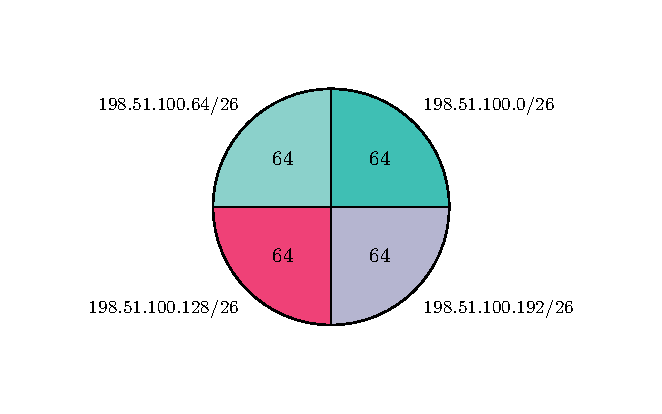
\includegraphics[width=\textwidth]{images/ip/subnetting.pdf}
\end{sidecaption}
\end{figure}

Let's start with the range 192.168.0.0/24.
The host part is eight bits in size so the range contains 256 \IP\ addresses.
Every time we add a bit to the network part, we split the range in two and thus half the number of available addresses per subnet.
If we change the prefix length to 25, we get two subnets each containing 128~addresses.
If we change the prefix length to 26, each of these two subnets gets halved again, all four parts containing 64~addresses.
When we make the prefix length 27~bits, we get eight subnets of 32~addresses each.

As you can see in \vref{fig:vlsm} you can take one subnet and divide it further into smaller parts.
In this case one of the four networks has been split again.
This is called \acf{VLSM}.

\begin{figure}
\begin{sidecaption}%
   [With \acs{VLSM} you can divide an \acs{IP} block in unequal parts]%
   {When using \acs{VLSM} you can further divide a subnet into smaller segments}%
   [fig:vlsm]
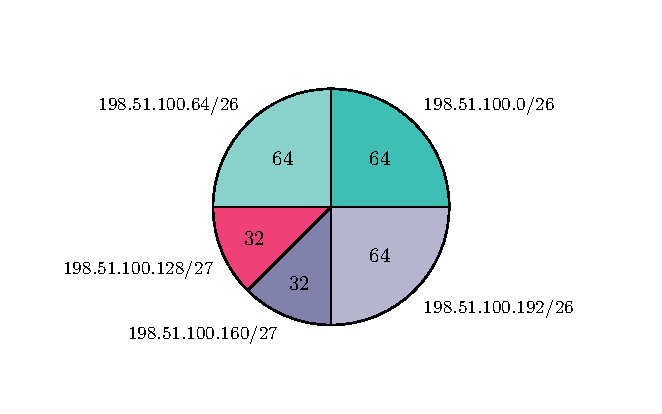
\includegraphics[width=\textwidth]{images/ip/vlsm.pdf}
\end{sidecaption}
\end{figure}


\paragraph{Why do we need subnetting?}
   \index{subnetting}
We are the network administrators of a small company.
We have a couple (50) of desktop computers for the employees, as well as a few (10) servers.
We contact \acs{RIPE} \acs{NCC}%
    \footnote{\gls{RIPE} \gls{NCC} is the \gls{RIR} for Europe, the Middle East and parts of central Asia. As a \gls{RIR}, it oversees the allocation and registration of internet number resources such as \acs{IP} addresses and autonomous system numbers.}
and tell them we need sixty \acs{IP} addresses, plus some extra just in case we will grow and need more computers.
Since a class~c address range contains 256~\acs{IP} addresses, \gls{RIPE} will give us one such range, e.g.~198.51.100.0/24.%
   \iacs{RIPE}

Now we have a problem.
We have plenty of \acs{IP} addresses but we need two separate networks.
Or perhaps we need three or even four.
Maybe we want to isolate the public internet-facing servers from the private servers that should not be reachable from the Internet.
We have received plenty of addresses, it is up to us to decide how to group them and to determine how large each network must be.

Remember that these different classes are just made-up methods of determining which part of the \acs{IP} address is the network number and which part is the host identifier.
\acs{IP} addresses themselves are just 32-bit numbers so we can group them any way we like.


\section{\acl{DHCP}}
\label{sec:ip-dhcp}


\paragraph{simplifies \acs{IP} address configuration}
   \iacs{DHCP}
Without the \gls{DHCP} you would have to contact a network administrator every morning at work when you power on your laptop and want to connect it to the (wireless) network.
Back at home or at a friend's place you need to change the \acs{IP} settings again, including which \acs{DNS} servers to use.
This requires huge lists with available \acs{IP} addresses which are being updated constantly with newly available \acs{IP} addresses -- should you remember to contact your network administrator before leaving work -- or available \acs{IP} addresses becoming unavailable as people come in to work every morning.%
   \footnote{%
      The first chapter of \textcite[3-7]{droms} gives a look in the life of a network administrator in the days when there was no \acs{DHCP} yet.
      I copied it to \vref{chap:dhcp-extract}.
   }

\paragraph{\acs{DORA}}
   \index{DHCP@\acs{DHCP}!DORA@\acs{DORA}}
\gls{DHCP} operations fall into four phases: server discovery, \acs{IP} address lease offer, lease request, and lease acknowledgement.
These stages (see \vref{fig:dora}) are often abbreviated as \acs{DORA} for \acl{DORA}.

\begin{figure}
\begin{sidecaption}{The foure stages of acquiring an \acs{IP} address from a \acs{DHCP} server}[fig:dora]
\centering
\tikzstyle{node}=[
    minimum width=20mm,
    minimum height=8mm,
    inner sep=0mm,
    font=\small\sffamily,
    text=black,
    node distance=12mm,
    draw=spot1,
    fill=spot1!20
]
\tikzstyle{arrow}=[->,>=stealth',semithick]

\begin{tikzpicture}

\node[node] (c) at (0,0) {client};
\node[node] (s) at (7,0) {server};

\draw [thick,arrow] (c) -- +(0,-4) node[below] {$t$};
\draw [thick,arrow] (s) -- +(0,-4) node[below] {$t$};

\node (start) at ($(c)-(0,1)$) {};

\draw [thick,arrow] (start.center) -- node[below] {\footnotesize discover} ++(7,-0.5);
\draw [thick,arrow,<-,spot2] ($(start)+(0,-1.2)$) -- node[below] {\footnotesize offer} ++(7,0.5);
\draw [thick,arrow] ($(start)+(0,-1.4)$) -- node[below] {\footnotesize request} ++(7,-0.5);
\draw [thick,arrow,<-,spot2] ($(start)+(0,-2.6)$) -- node[below] {\footnotesize acknowledge} ++(7,0.5);
\end{tikzpicture}
\end{sidecaption}
\end{figure}

\paragraph{lease time}
   \index{DHCP@\acs{DHCP}!lease time}
When the server offers the client an \acs{IP} address, it does this for a specific lease time.
After this time expires, the client must relinquish the given \acs{IP} address.
To prevent the client from getting disconnected from the network while it requests a new \acs{IP} address, it can refresh the lease on its current \acs{IP} address midway the lease period.

For example, when the client gets an \acs{IP} address with a lease time of eight hours, it can refresh the lease period after four hours.
If the server grants this request, the lease is again valid for eight hours.

If the \acs{DHCP} server denies the request, the client loses the lease right away.
It cannot use the \acs{IP} address for the remaining four hours but must send a \acs{DHCP} discover message to request a new \acs{IP} address.

\paragraph{\acs{DHCP} relay}
   \index{DHCP@\acs{DHCP}!relay}
As it is impractical to configure a \acs{DHCP} server on each network, routers can be configured to act as \acs{DHCP} relays, forwarding the broadcast messages%
   \fxwarning{Explain why \acs{DHCP} uses broadcast messages.}
as unicast to a remote \acs{DHCP} server.

\paragraph{reservations}
A \acs{DHCP} server can be configured such to always provide the same client (\acs{MAC} address) the same \acs{IP} address.
This way the client practically has a fixed \acs{IP} address, as if configured manually on the device itself.
But you keep the \acs{IP} address configuration on a central location.




\section{\Acl{NAT}}
\label{sec:ip-nat}


\paragraph{private \acs{IP} space}
There is nothing special about `private' \acs{IP} addresses.
   \index{IP address@\acs{IP} address!private}
   \index{IP address@\acs{IP} address!public}
   \index{internet}
   \iacs{ISP}
They are not treated any different from `public' \acs{IP} addresses by routers or end hosts.
The only difference is that they \emph{should} not be routed on the public internet.
This means that \acl{ISP} should block packets with a private \acs{IP} address as either the source or the destination address.

There are several blocks of private \acs{IP} addresses which can be used internally by organisations without having to ask for permission to do so.
\begin{multicols}{2}
\raggedcolumns
\begin{itemize}
\item 10.0.0.0/8
\item 100.64.0.0/10
\item 169.254.0.0/16
\item 172.16.0.0/12
\item 192.0.2.0/24
\item 192.168.0.0/16
\item 198.18.0.0/15
\item 198.51.100.0/24
\item 203.0.113.0/24
\end{itemize}
\end{multicols}

The ranges 10.0.0.0/8, 172.16.0.0/12, and 192.168.0.0/16 were introduced as private IP ranges to enable \acf{NAT}.
The ranges 192.0.2.0/24, 198.51.100.0/24, and 203.0.113.0/24 have been reserved for documentation purposes but can be used internally within an organisation.
The range 100.64.0.0/10 was added in 2012 for use in carrier-grade \ac{NAT} scenarios (\rfc{6598}):

\begin{quote}
Shared-address space is distinct from \rfc{1918} private-address space because it is intended for use on service-provider networks.
However, it may be used in a manner similar to \rfc{1918} private-address space on routing equipment that is able to do address translation across router interfaces when the addresses are identical on two different interfaces.
\end{quote}

The address range 169.254.0.0/16 is a special case.
These are defined as `link-local' addresses and must not be forwarded by a router as these addresses are not guaranteed to be unique beyond their network segment.%
   \index{IP address@\acs{IP} address!link-local}
Microsoft names this range \acp{APIPA}.%
   \index{IP address@\acs{IP} address!APIPA@\acs{APIPA}}
A \acs{DHCP}\iacs{DHCP} client takes a random \acs{IP} address from this range when it receives no responses from any \acs{DHCP} server.

\paragraph{port-based address translation}
   \iacs{NAT}
The majority of network address translators map multiple private hosts to one publicly exposed \acs{IP} address.
In a typical configuration, a local network uses one of the designated private \acs{IP} address subnets (\rfc{1918}).
One or more routers sit at the border of this private network connecting it to the public Internet.

As traffic passes from the local network to the Internet, the source address in each packet is translated on the fly from its private address to the public address of the router.
The router tracks basic metadata about each active connection (particularly the destination address and port).
When a reply returns to the router, it uses the connection tracking data it stored during the outbound phase to determine the private address on the internal network to which to forward the reply.

All \acs{IP} packets have a source \acs{IP} address and a destination \acs{IP} address.
Typically packets passing from the private network to the public network will have their source address modified, while packets passing from the public network back to the private network will have their destination address modified.
To avoid ambiguity in how replies are translated, further modifications to the packets are required.
For \acs{TCP} and \acs{UDP} the port numbers are changed so that the combination of \acs{IP} address and port number on the returned packet can be unambiguously mapped to the corresponding private network destination.
\rfc{2663} uses the term \gls{NAPT} for this type of \acs{NAT}.
Other names include \gls{PAT}, \acs{IP} \emph{masquerading}, \acs{NAT} \emph{overload} and \emph{many-to-one} \acs{NAT}.
This is the most common type of \acs{NAT} and has become synonymous with the term \acs{NAT} in common usage.
   \index{IP masquerading@\acs{IP} masquerading}
   \index{NAT@\acs{NAT}!overload}
   \index{NAT@\acs{NAT}!many-to-one}
   \iacs{PAT}

\paragraph{pool of public addresses}
   \index{NAT@\acs{NAT}!pool}
It is possible to use multiple public \acs{IP} addresses to translate the private \acs{IP} address into.
When this is used in combination with port-based address translation, it allows for multiple thousands of private hosts to communicate on the Internet.

% TODO: either explain more, or delete?
\paragraph{one-to-one translation}
   \index{NAT@\acs{NAT}!static}
   \index{NAT@\acs{NAT}!one-to-one}
This method is most often used to translate a range of private \acs{IP} addresses into a different range of private \acs{IP} addresses.
This is often needed when two companies with overlapping \acs{IP} address space connect their networks together.




\section{\Acl{ICMP}}
\label{sec:ip-icmp}

The \acf{ICMP} is a supporting protocol in the internet protocol suite.
It is used by network devices, including routers, to send error messages and operational information indicating success or failure when communicating with another \acs{IP} address, for example, an error is indicated when a requested service is not available or that a host or router could not be reached.

The program \cmd{ping} uses \acs{ICMP} to detect whether the destination is reachable and alive.
It sends out an \acs{ICMP} echo request (\cref{tab:icmp}) and expects to receive an \acs{ICMP} echo reply from the destination.
Receiving this reply tells us two things:
\begin{itemize}
\item
   the destination host is turned on and connected to the network as it was able to receive our message and reply to it;
\item
   the network between our computer and the destination is working as all the devices in the middle were able to send our request to the destination as well as send its reply back to us.
\end{itemize}

\begin{table}
\begin{sidecaption}{Most common \acs{ICMP} types and codes}[tab:icmp]
\centering
\begin{tabular}{rrl}
{type} & {code} & {description} \\
\midrule
 0 &  0 & echo reply \\
 3 &  0 & destination network unreachable \\
 3 &  1 & destination host unreachable \\
 3 &  2 & destination protocol unreachable \\
 3 &  3 & destination port unreachable \\
 3 &  4 & fragmentation needed but \SC{DF}-bit set \\
 3 & 13 & communication administratively prohibited \\
 5 &  0 & redirect datagram for the network \\
 5 &  1 & redirect datagram for the host \\
 8 &  0 & echo request \\
11 &  0 & \acs{TTL} expired in transit \\
\end{tabular}
\end{sidecaption}
\end{table}

If we do not receive a reply from the end host it can be because of one or more issue in the network.
\begin{itemize}
\item
   The end host could be turned off, have a firewall configured which prohibits sending or receiving \acs{ICMP} messages, or have an incorrect gateway configured so that the reply cannot reach us.
\item
   A network firewall in the path between source and destination can prevent the \acs{ICMP} query from reaching the destination.
   It could also prevent the reply form reaching us.
\item
   The destination network could be unknown to one of the routers in the path preventing the query from reaching its destination.
   Our own network could also be unknown to one of the routers in the path preventing the reply from reaching us.
\end{itemize}
More troubleshooting is needed to determine the exact problem or problems so that they can get fixed.
A good place to start would be to use the program \cmd{traceroute} (on Windows it is called \cmd{tracert}).

\fxwarning{Complete this section.}


\paragraph{path \acs{MTU} discovery}

See also \emph{time-to-live} on p.~\pageref{par:ip-ttl} and \emph{fragmentation} on p.~\pageref{par:ip-fragmentation}.
\fxwarning{Complete this section.}



\section{\acs{IP} header}
Before we delve into the second major topic, \IP\ routing, let's first take a look at the \IPfour\ packet header.

\begin{figure}
\begin{sidecaption}{The \IPfour\ packet header}[fig:ipv4-header]
\centering
\begin{bytefield}{32}
\bitheader{0,3,4,7,8,13-15,16,18,19,31}\\
\bitbox{4}{version}
\bitbox{4}{\SC{IHL}}
\bitbox{6}{\SC{DSCP}}
\bitbox{2}{\footnotesize\SC{ECN}}
\bitbox{16}{total length} \\
\bitbox{16}{identification}
\bitbox{3}{flags}
\bitbox{13}{fragment offset} \\
\bitbox{8}{\acs{TTL}}
\bitbox{8}{protocol}
\bitbox{16}{checksum} \\
\wordbox{1}{source \IP\ address} \\
\wordbox{1}{destination \IP\ address} \\
\wordbox[tlr]{1}{options}\\
\skippedwords \\
\wordbox[blr]{1}{}\\
\end{bytefield}
\end{sidecaption}
\end{figure}

Most fields are not important to us but a few are.
\begin{description}
\item[source \IP\ address]
   The \IP\ address of the end host sending the packet.
\item[destination \IP\ address]
   The \IP\ address of the end host to which we want to send the packet.
\item[\acf{TTL}]
   The source puts a value (0-255) in this 8-bit field and every router forwarding the packet first decrements this value by one.
   When the number reaches zero, the packet is discarded.
   This is a simple method to prevent loops in the network where packets travel endlessly in a circle between two or more routers.
\item[protocol]
   The value in this 8-bit determines the contents of the packet.
   This value tells the operating system receiving the packet from the network to which higher-level protocol to send the data.
\item[checksum]
   A checksum of the header is calculated and stored in this field.
   The receiver calculates the checksums and compares it to this value.
   If both values are the same, the receiver can assume the data to be correct.
   If both checksums differ, the packet has been corrupted in transit and is discarded.
\end{description}

\begin{margintable}
\begin{tabular}{rl}
 1 & \acs{ICMP}  \\
 6 & \acs{TCP}   \\
17 & \acs{UDP}   \\
47 & \acs{GRE}   \\
50 & \acs{ESP}   \\
51 & \acs{AH}    \\
88 & \acs{EIGRP} \\
89 & \acs{OSPF}  \\
\end{tabular}
\caption{A few important \IP\ protocol values.}
\end{margintable}

\IPfour\ options are not often used and some can even be dangerous.
Many networks are configured to drop packets with either the \emph{Loose source and record route} option or the \emph{Strict source and record route} option.

In \IPsix\ options are implemented as extensions.
For example the IPsec \acf{AH} and \acf{ESP} headers are implemented as \IPsix\ extension headers.
   \index{VPN@\acs{VPN}!IPsec}
Fragmentation is also implemented using an extension header although \IPsix\ packets are not supposed to be fragmented.


\section{Routing}
\label{sec:ip-routing}

\paragraph{What is a router?}
   \index{router}
   \index{packet!forwarding}
A router is really just a specialised computer that \emph{forwards} packets it receives but which are not destined for itself.
A computer can also be configured to function as a router by turning on this option (\vref{lst:freebsd-enable-routing,lst:rhel-enable-routing}).


\begin{fltlisting}[h!]
\begin{sidecaption}{Enable routing on a FreeBSD host}[lst:freebsd-enable-routing]
\begin{lstlisting}
# sysrc gateway_enable="YES"
# sysctl net.inet.ip.forwarding=1
\end{lstlisting}
\end{sidecaption}
\end{fltlisting}

\begin{fltlisting}[h!]
\begin{sidecaption}{Enable routing on a \acs{RHEL} host}[lst:rhel-enable-routing]
\begin{lstlisting}
# echo "net.ipv44.ip_forward=1" >> /etc/sysctl.conf
# echo 1 > /proc/sys/net/ipv4/ip_forward
\end{lstlisting}
\end{sidecaption}
\end{fltlisting}

\fxwarning{These new listings don't play nice with \textbackslash{}vref.}

When a router receives a packet with a destination \acs{IP} address which does not belong to any of the router's interfaces, the router looks up the \acs{IP} address in its \emph{routing table} and forwards the packet out the given interface.%
   \index{routing table}

\begin{fltlisting}[h!]
\begin{sidecaption}{The routing table on a linux machine}[fig:routing-table]
\begin{lstlisting}
[doyle] ~ $ netstat -rn
Kernel \acs{IP} routing table
Destination     Gateway         Genmask         Iface
10.0.0.0        172.24.12.1     255.255.240.0   eth1
10.0.16.0       172.24.12.1     255.255.240.0   eth1
10.0.32.0       192.168.16.1    255.255.224.0   eth2
172.21.3.0      0.0.0.0         255.255.255.0   eth0
172.24.12.0     0.0.0.0         255.255.255.0   eth1
192.168.16.0    0.0.0.0         255.255.255.0   eth2
0.0.0.0         172.21.3.1      0.0.0.0         eth0
\end{lstlisting}
\end{sidecaption}
\end{fltlisting}

Routers only know about the networks they directly connect to.
They must thus learn about distant networks.
This can happen in one of two ways, either the network administrator manually configures the router to forward a certain prefix to some other router (the \emph{next-hop} router) or the routers in a network can use a \emph{dynamic routing protocol} to teach each other about the networks they know and how to reach them.
   \index{router!next-hop}

\begin{marginfigure}
\noindent
\fxwarning[layout=inline]{Insert a figure here.}
\caption{Router $R_1$ knows about networks~1 and~2, but not about network~3.}
\label{fig:ip-local-networks}
\end{marginfigure}

\paragraph{\acl{TTL}}
\label{par:ip-ttl}
   \iacs{TTL}
The \acs{IP} header contains a \gls{TTL} field which indicates how many routers (hops) it can pass before it must be deleted.
This prevents the data packet from circulating indefinitely.
As it is an 8-bit field, the maximum value is~255 but a recommended initial value is~64.\footnote{See \rfc{1700}, p.~64.}

As it does not really signify some time spent in transit, with the development of \acs{IP} version~6, they changed the name of this field to \emph{hop limit} as that is what it really does: limit the number of hops (routers) that a packet can travel.


\paragraph{fragmentation}
\label{par:ip-fragmentation}
   \index{fragmentation}
   \iacs{MTU}
Different physical media have different maximum frame sizes.
For example, Ethernet has a maximum frame size of 1518~bytes or a \gls{MTU} of 1500~bytes, which is the frame size minus the header length.
Token Ring has a much larger \gls{MTU} of 4464~bytes, \gls{ATM} and \SC{X.25} have much smaller \acp{MTU} of 48~and 576~bytes respectively.

When a router connects an Ethernet segment to an \gls{ATM} circuit, it must \emph{fragment} the 1500-byte frames it receives into 48-byte cells that it can forward across the \ac{ATM} network.
Once fragmented, routers do not reassemble the pieces back together as they might take different paths through the network and are not guaranteed to arrive in the correct order.
The end host is responsible for piecing all fragments back together.

Another example when fragmentation is being used, is in the communication between a data centre and campus network as the former often uses jumbo frames (an \acs{MTU} of 9000~bytes) while the latter uses normal Ethernet frames which have an \acs{MTU} of 1500~bytes.%
   \index{frame!jumbo}
   \index{data centre}

Finally, you will also encounter fragmentation on IPsec \aclp{VPN} where the maximum transmission unit is slightly smaller than the normal 1500~bytes.
   \index{VPN@\acs{VPN}!IPsec!fragmentation}

\paragraph{broadcast domain}
   \index{broadcast domain}
A \emph{broadcast domain} is that part of the network to which a broadcast messages propagates.
One of the functions of a router is to stop broadcasts, not forwarding the to other parts of the network.

\paragraph{static routing}
   \index{static routing}
Static routing is a form of routing that occurs when a router uses a manually-configured routing entry, rather than information from dynamic routing traffic.
In many cases, static routes are manually configured by a network administrator by adding in entries into a routing table, though this may not always be the case.
Unlike dynamic routing, static routes are fixed and do not change if the network is changed or reconfigured.
Static routing and dynamic routing are not mutually exclusive.
Both dynamic routing and static routing are usually used on a router to maximise routing efficiency and to provide backups in case dynamic routing information fails to be exchanged.
Static routing can also be used in \emph{stub networks},%
\index{stub network}%
\footnote{%
A stub network is a (part of a) network with only one way to reach the rest of the network.
It thus does not need detailed knowledge about the network but can usually route all traffic using a single default route pointing to the exit point.
}
or to provide a gateway of last resort.


\paragraph{dynamic routing protocols}
   \index{routing protocol!distance-vector}
   \index{routing protocol!link-state}
\begin{description}
\item[distance-vector]
A distance-vector routing protocol is like putting signposts on every crossroads with the router being the crossroads.
Every router learns about all networks but only the direction it has to send traffic to (the next-hop router) and the total distance to reach the remote network.
\item[link-state]
A link-state routing protocol is comparable to every router building a roadmap with all links interconnecting the different routers included.
Once the entire map has been drawn, each router can calculate the best path to reach each destination.
\end{description}

\paragraph{metric}
   \index{metric}
When we take a look at \vref{fig:metric}, we see that router $R_4$ connects to the network 192.0.2.0/24.
It advertises this to routers $R_2$ and $R_3$ which in turn both advertise this network to router $R_1$.
Router $R_1$ now knows two paths to reach the destination network 192.0.2.0/24, once via $R_2$ and once via $R_3$.
For $R_1$ to decide which path is best, it compares the \emph{metric} of both paths; the lowest value is the best path.

When a router advertises a network, it includes a metric value.
When another router forwards this information -- e.g.~router $R_2$ forwards the information about network 192.0.2.0/24 to router $R_1$ -- it updates the metric value.

Every routing protocol can use a different metric.
\acs{RIP} uses a simple \emph{hop count} or the number of routers you have to traverse to reach your destination.
\acs{OSPF} and \acs{IS-IS} use a generic \emph{cost} value.
Most \acs{OSPF} implementation use a cost value based on the bandwidth of the links while with \acs{IS-IS} the network administrator has to manually set a cot value for each link.
\acs{EIGRP} uses a very complex formula to determine the metric, see \vref{eqn:eigrp-metric}.

\begin{figure}
\begin{sidecaption}[The metric decides the best route in a network]{A router can learn a prefix from several other routers. The metric decides the best route.}[fig:metric]
\centering
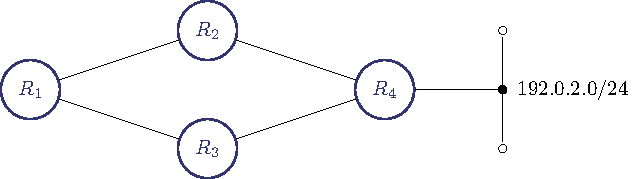
\includegraphics[width=\textwidth]{images/ip/metric.pdf}
\end{sidecaption}
\end{figure}


\paragraph{equal-cost multi-path routing}
   \iacs{ECMP}
   \index{load balancing!network}
If both $R_2$ and $R_3$ advertise the same metric towards $R_1$ both paths are equally good and $R_1$ \emph{load balances} traffic over both paths.
The router uses an algorithm to send roughly fifty percent of packets via $R_2$ and the other fifty percent via~$R_3$.

\paragraph{administrative distance}
   \index{administrative distance}
The \emph{metric} indicates the preference of a single route learnt from different routers via the same routing protocol.
It is however also possible for a router to learn a route from different routing protocols.
The \emph{administrative distance} gives the preference or credibility of a routing protocol over another.
For example, on Cisco routers the administrative distance or credibility of \acs{RIP} is~110 while the administrative distance of \acs{OSPF} is~90.
As lower values are preferred, when a router running both \acs{RIP} and \acs{OSPF} learn about the same route from both protocols, it will prefer the route learnt from \acs{OSPF} over the route learnt from \acs{RIP}.%
   \footnote{%
      The administrative distance is -- as the name implies -- a purely administrative value, meaning the network administrator chooses which routing protocol to prefer over the other.
      However, as a best practice a network should only use a single routing protocol.
      It is not good to combine several routing protocols as the network then becomes needlessly complex and error prone.
   }

\paragraph{\acf{RIP}}
The \acl{RIP} is an example of a distance-vector routing protocol using the \emph{hop count} or the number of routers to count how good a given path is.%
   \index{metric!hop count}
It is a very simple protocol useful in smaller networks.
The protocol is not suitable for larger networks because of its slow \emph{convergence time} and its tendency to propagate good information slowly and negative information quickly.
   \index{convergence time}

\paragraph{route poisoning}
   \index{route poisoning}
% source: https://www.geeksforgeeks.org/route-poisoning-and-count-to-infinity-problem-in-routing/
The main issue with distance-vector routing protocols is routing loops.%
   \fxwarning{Briefly explain routing loops.}
   \index{routing loop}
This routing loop in the network causes the count-to-infinity problem.%
   \fxwarning{Briefly explain the count-to-infinity problem.}
   \index{count-to-infinity}
Routing loops usually occur when an interface goes down or two routers send updates at the same time.

Route poisoning helps to alleviate this problem by advertising the route back to its source with a metric of infinity.
This ensures that the router originally advertising the prefix can never use its neighbours to reach the given network.

\paragraph{split horizon}
   \index{split horizon}
Split horizon is another method to prevent routing loops from occuring.%
   \index{routing loop}
This time, instead of advertising the routes back with a metric of infinity, we simple do not advertise the route back to where we learned it from.
This method is not as good as using route poisoning to prevent routing loops.
Logically you can not use both both methods. Either you use neither method, or you use one or the other.

\paragraph{hold-down timer}
   \index{hold-down timer}
When a router receives a routing update advertising a network to be unreachable, it starts a hold-down timer.
Until the timer expires, the router will discard any subsequent route messages that indicate the route is in fact reachable.
It can solve the case where multiple routers are connected indirectly.
There are realistic scenarios where split horizon and split horizon with poisoned reverse can do nothing.%
\fxwarning{This is very vague.}

\paragraph{\acl{EIGRP}}
   \iacs{EIGRP}
The \acf{EIGRP} was a Cisco proprietary protocol which has been made publicly available in 2013 but has not been implemented by other vendors.

While \acs{RIP} and \acs{OSPF} have a very simple metric, \acs{EIGRP} has a rather complex one.
The metric $m$ is calculated as such:
\begin{equation}
m = \left[\left(k_1 B_m  + k_2 \frac{B_m}{256-L} + k_3 D_s\right) \times \frac{k_5}{k_4 + R}\right] \times 256,
\label{eqn:eigrp-metric}
\end{equation}
with $B_m$ being the minimum bandwidth along the path to the destination, $D_s$ being the total delay along the path, $L$ and $R$ being the load an the reliability of the link respectively, taken over a five-minute interval.
The five $k$ values are user-configurable weights to each part of the equation.%
   \footnote{%
      My advice is to change these $k$ values to exclude the bandwidth from the equation.
      Altering the bandwidth value also changes the calculations for \acs{QOS} among other things while the delay value is used only by \acs{EIGRP}.
      This will result in more readable metrics and it will be easier to tune \acs{EIGRP} without interfering with other services on the router.
      See the exercises on how to do this.
   }

As if \cref{eqn:eigrp-metric} is not complex enough, there are a few important caveats.
The minimum bandwidth $B_m$ is calculated by dividing a reference bandwidth of \SI{1e7}{\bit\per\second} by the smallest configured bandwidth on the interfaces along the path.
It does not take into account the actual bandwidth of an interface, but the setting configured on the interface.

The total delay also is not measured along the path but fixed values are used depending on the interface type.
A serial interface always has a default delay of \SI{20000}{\micro\second} while a Gigabit Ethernet interface has a default delay of \SI{10}{\micro\second}, regardless of the length of the cable.
Both settings are user configurable.
The value $D_s$ is measured in tens of microseconds so for a serial interface the value 2000 would be used instead of \numprint{20000}.

\begin{margintable}
\begin{tabular}{lr}
serial   & {20000} \\
\SC{T1}  & {20000} \\
Ethernet & 1000  \\
FastE    & 100   \\
GigE     & 10    \\
10GigE   & 10    \\
\end{tabular}
\caption{Default delay values per interface type}
\label{tab:ip-intf-delay}
\end{margintable}

If load an reliability are used in the computation -- which by default they are not -- the initial values are set during peer establishment and do not change dynamically with the router.
These values are a remnant of an older version of the protocol where they did change with every update to reflect the live status of the network.

Finally, when $k_5=0$, instead of the entire equation to become zero, this factor is removed from the equation.

\paragraph{\acf{OSPF}}
   \iacs{OSPF}
The \acl{OSPF} protocol is a link-state routing protocol suitable for small network all the way up to massive service provider networks.
It can scale to very large networks because of the introduction of a concept called \emph{areas}, used to divide the entire network into smaller, more manageable parts.

The \acs{OSPF} metric $m$ is calculated by summing all costs along the path with the cost being a reference bandwidth devided by the actual bandwidth $B_i$ of the link.

\begin{margintable}
\begin{tabular}{lr}
\SC{T1}  & 64      \\
Ethernet & 10      \\
FastE    & 1       \\
GigE     & 1       \\
10GigE   & 1       \\
\end{tabular}
\caption{Default \acs{OSPF} cost values per interface type}
\label{tab:ip-ospf-cost}
\end{margintable}

\begin{equation}
m = \sum_i\frac{10^8}{B_i}
\end{equation}

As you can see in \vref{tab:ip-ospf-cost} \acs{OSPF} by default cannot differentiate between a FastEthernet link at \SI{100}{\mega\bit\per\second} or a 10GigE link, while it clearly should!
Thus it is very important that you change the refence bandwidth on \emph{all} your routers in the network to a value higher than your highest network link (see the practice questions).


\paragraph{\acf{BGP}}
   \iacs{BGP}
   \index{routing protocol!path-vector}
   \index{autonomous system}
The \acl{BGP} is neither a distance-vector nor a link-state routing protocol.
It is the only \emph{path-vector} routing protocol and it is used to interconnect different \emph{autonomous systems}, meaning it can be used to interconnect networks operated by different organisations.
A basic \acs{BGP} configuration is relatively simple but it can quickly become extremely complex.

Contrary to normal routing protocols which serve to make all networks known within the entire internetwork, \acs{BGP} aims to limit reachability and focusses on \emph{policies}.
You can tweak the protocol so that you can exactly control the path a packet has to travel through the network to reach its destination.



\section{Review questions}
\label{sec:ip-review-questions}
\fxwarning{I should probably differentiate between review questions for the theory course, guided exercises for the extra hands-on course and practice questions for students to do at home.}

\begin{enumerate}
\item
   Given the network 100.65.0.0/16, give the network address, broadcast address, and the first and last available \IP\ addresses.
\item
   Given the network 198.19.0.0/24, give the network address, broadcast address, and the first and last available \IP\ addresses.
\item
   Given the network 203.0.113.32/27, give the network address, broadcast address, and the first and last available \IP\ addresses.
\item
   How many available or usable \IP\ addresses are there in the network 192.168.12.128/25?
\item
   Which class of \IP\ addresses provides a maximum of only 254 host addresses per network \SC{ID}?
   \begin{multicols}{2}
   \raggedcolumns
   \begin{enumerate}
   \item class a
   \item class b
   \item class c
   \item class d
   \item class e
   \end{enumerate}
   \end{multicols}
\item
   Given the \IP\ range 192.0.2.64/26, split this range up into four smaller blocks.
   Give the network and broadcast address for each of these four subnetworks.
\item
   What is the maximum number of \IP\ addresses that can be assigned to hosts on a local subnet that uses the 255.255.255.224 subnet mask?
   \begin{multicols}{2}
   \begin{enumerate}
   \item 14
   \item 15
   \item 16
   \item 30
   \item 31
   \item 62
   \end{enumerate}
   \end{multicols}
\item
   What is the subnetwork address for a host with the \IP\ address 200.10.5.68/28?
   \begin{multicols}{2}
   \begin{enumerate}
   \item 200.10.5.56
   \item 200.10.5.32
   \item 200.10.5.64
   \item 200.10.5.0
   \end{enumerate}
   \end{multicols}
\item
   You want to implement a mechanism that automates the \IP\ configuration, including \IP\ address, subnet mask, default gateway, and \acs{DNS} information.
   Which protocol will you use to accomplish this?
   \begin{multicols}{2}
   \begin{enumerate}
   \item \acs{SMTP}
   \item \acs{ARP}
   \item \acs{DHCP}
   \item \acs{SNMP}
   \end{enumerate}
   \end{multicols}
\item
   You have an interfaces on a router with the \IP\ address of 192.168.192.10/29.
   What is the broadcast address the hosts will use on this \acs{LAN}?
   \begin{multicols}{2}
   \begin{enumerate}
   \item 192.168.192.15
   \item 192.168.192.31
   \item 192.168.192.63
   \item 192.168.192.127
   \item 192.168.192.255
   \item 192.168.255.255
   \end{enumerate}
   \end{multicols}
\item
   To test the \IP\ stack on your local host, which \IP\ address would you ping?
   \begin{multicols}{2}
   \begin{enumerate}
   \item 127.0.0.0
   \item 1.0.0.127
   \item 127.0.0.1
   \item 127.0.0.255
   \item 255.255.255.255
   \end{enumerate}
   \end{multicols}
\item
   Which two of the following are private \IP\ addresses?
   \begin{multicols}{2}
   \begin{enumerate}
   \item 25.7.0.1
   \item 172.33.194.4
   \item 169.172.19.93
   \item 172.19.25.54
   \item 192.168.77.12
   \item 203.0.113.7
   \end{enumerate}
\end{multicols}
\end{enumerate}

\section{Guided exercises}
\label{sec:ip-guided-exercises}

\section{Practice questions}
\label{sec:ip-practice-questions}
\begin{enumerate}
\item
   Create a small network with a router, a switch and two computers.
   Configure the router's interface with the \IP\ address 192.168.0.1/26 and configure a \acs{DHCP} server so that the computers automatically get an \IP\ address when they power on.
   One computer should always get the \IP\ address 192.168.0.7.
\item
   Set up a small network with a few routers and configure \acs{EIGRP} as the routing protocol between them.
\item
   Change the $k$ values so that only the interface delay is used to calculate the metric.
\item
   Set up a small network with a few routers and configure \acs{OSPF} as the routing protocol between them.
\item   
\label{ex:ip-ospf-ref-bw}
   Change the reference bandwidth for \acs{OSPF} to match \SI{100}{\giga\bit\per\second}.
\end{enumerate}



\section{Further reading}
\label{sec:ip-reading}
\textcite{lammle-ccna,lammle-comptia} are both good resources to continue from here.
They both explain \acs{IP} addresses, subnetting, \acs{DHCP}, and routing in more detail.
Another great resource is \textcite{stevens} but this masterpiece is probably a bit too in-depth.
\textcite{doyle} is another classic.
The first volume focusses on the routing protocols \acs{RIP}, \acs{OSPF}, and \acs{IS-IS} while the second volume covers \acs{BGP}.